\documentclass[a4paper]{article}

%\usepackage{texments}
\usepackage{graphicx}
\usepackage{caption}
\usepackage{subcaption}
\usepackage{tabularx}
\usepackage{booktabs}
\usepackage[table]{xcolor}
\usepackage{minted}
\usepackage{amsmath}

\usepackage[left=2.5cm, right=2.5cm, bottom=2.5cm,footskip=.5cm, top=2.5cm]{geometry}


\usepackage[utf8]{inputenc}
\usepackage[T1]{fontenc}
\usepackage[ngerman]{babel}

\definecolor{bg}{rgb}{0.950,.95,0.95}
\newminted{pycon}{bgcolor=bg,linenos=false,tabsize=4}

\begin{document}

%%%%%%%%%%%%%%%%%%%%%%%%%%%%%%%%%%%%%%%
%%% 6.1                             %%%
%%%%%%%%%%%%%%%%%%%%%%%%%%%%%%%%%%%%%%%

\section*{Aufgabe1}
\subsection*{(1a)}
treap.py
\subsection*{(1b)}
treap.py
\subsection*{(1c)}
Implementierung in treap.py (es wird auch geprüft, dass beide Bäume die gleichen Elemente in gleicher Sortierung enthalten). Im standard ouput werden die ersten 7 Ebenen ausgegeben.
\subsection*{(1d)}
Ein perfekt ausbalancierter Baum hätte die Tiefe 13 (vgl. standard output). Die Anzahl der Nodes wäre gleich wie im random bzw. dynamic Treap. Daraus lässt sich über $d \le \log_2(N) < d+1$ bestimmen, wobei $N$ die Zahl der Nodes und $d$ die Tiefe ist. Die Anzahl der Nodes ist 13658 (vgl. standard output). Die Tiefe des random Treaps schwankt, da die Prioritäten random vergeben werden. Die Tiefe ist immer kleiner als die des dynamic Treaps, jedoch noch deutlich vom balanced Tree entfernt. Die Tiefe des dynamic Treaps ist konstant bei 38. (vgl. Tabelle \ref{tab:depth})
\begin{table}[H]
\centering
\begin{tabular}{|c|c|c|}
\hline
balanced & random & dynamic \\\hline
$13$ & $33\pm2$ & $38$ \\\hline
\end{tabular}
\caption{Tiefe der verschiedenen Trees/Treaps}
\label{tab:depth}
\end{table}

Die mittlere Zugriffszeit beim dynamic Treap ist kürzer als beim random Treap. Bei letzterem variiert sie, da der random Treap nicht bei jedem Programmdurchlauf identisch ist. Die Zugriffszeiten beim random Treap sind ca. 1.5 mal so hoch wie beim dynamic Treap (vgl. standard output).


\section*{Aufgabe 2}
\subsection*{(2 a)}
Da die Punkte gleichverteilt sind, ist die Verteilung der Punkte mit Radius $r$ gegeben durch das Volumenverhältnis 
\begin{equation}
F(r)=\frac{\pi r^2}{\pi}.
\end{equation}
Die Dichtefunktion ist daher
\begin{equation}
f(r)=\frac{dF(r)}{dr}=2r.
\end{equation}
Nun sucht man Intervallgrenzen $r_j$, so dass Punkte im Intervall $[r_j,r_{j+1})$ auf den Index $j$ abgebildet werden. Die Intevallgrenzen sollen so gewählt werden dass im Schnitt in allen Intevallen gleich viele Punkte sind.
Die Anzahl der Punkte im Bucket $i$ ist gegeben durch
\begin{equation}
N_i = \int_{r_i}^{r_{i+1}}2r dr = r_{i+1}^2-r_i^2.\label{eq:N}
\end{equation}
Es muss also gelten $N_i=N_{i+1}$. Mit~\eqref{eq:N} folgt daraus für die Intervallgrenzen $r_{i+2}^2=2r_{i+1}^2-r_i^2$. Daraus folgt $r_i=\sqrt{i}\cdot r_1$. Diese Intervallgrenzen werden realisiert indem man die Indexfunktion
\begin{equation}
index_{quad}(r)=\lfloor r^2M\rfloor
\end{equation}
wählt.

\subsection*{(2b)}
Die Funktion testUniformity gibt $\tau$ zurück. Für die Arraygrößen $10^2,10^3,10^4,10^5,10^6$ und M=$2,4,8,20,100$ wurde getestet ob $\tau>3$ (nicht gleichverteilt). Die Indexfunktion $\lfloor r^2M\rfloor$ besteht alle $25$ Tests, die Indexfunktion $\lfloor rM\rfloor$ besteht nur $1-2$ von 25 Tests.




\subsection*{(2c)}

Die Laufzeit von bucketSort scheint linear zu sein, siehe Abbildung~\ref{fig:runtime}. Die Laufzeit unter Verwendung von $\lfloor rM\rfloor$ ist geringer als die Laufzeit unter Verwendung von $\lfloor r^2M\rfloor$. Dies Widerspricht der Erwartung. Die Vorteile durch Verwendung von $\lfloor r^2M\rfloor$ (gleichmäßig gefüllte Buckets) könnten geringer sein als der Mehraufwand (quadrieren, $r^2$)?

\begin{figure}
  \centering
  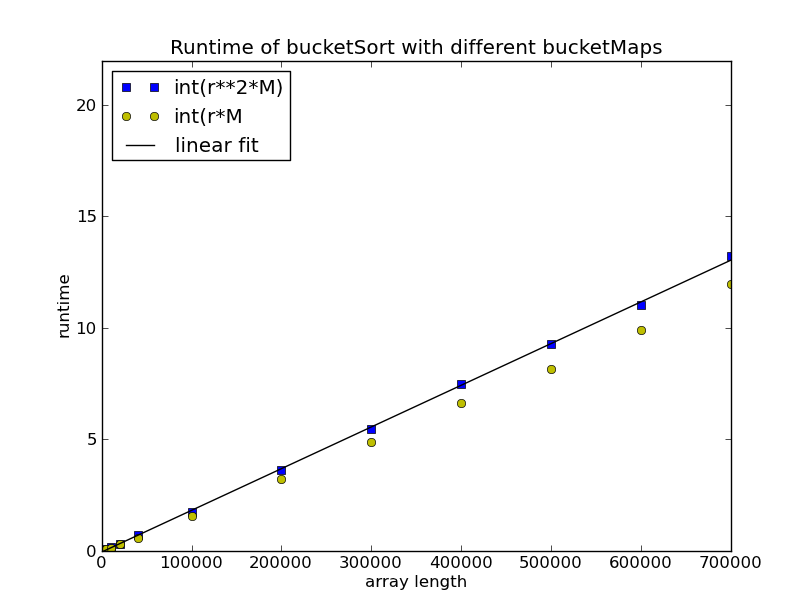
\includegraphics[width=10cm]{runtime.png}
  \caption{Laufzeit von BucketSort unter Verwendung der zwei bucketMaps.}
  \label{fig:runtime}
\end{figure}



\end{document}
